\documentclass[leqno]{article}
\usepackage[utf8]{inputenc}
\usepackage{enumitem}
\usepackage{tikz}
\usepackage[parfill]{parskip} % Don't start new paragraph with tab.
\usepackage{amsmath} % For \tag and \eqref

\title{Computationele logica}
\author{
    Kamans, Jim\\
    \texttt{10302905}
    \and
    Roosingh, Sander\\
    \texttt{11983957}
    \and
    Schenk, Stefan\\
    \texttt{11881798}
}
\date{November 2017}

\begin{document}

\maketitle


%%%%%%%%%%%%%%%%
%% Exercise 1 %%
%%%%%%%%%%%%%%%%
\section*{Exercise 1}

\begin{enumerate}

    \item The sentence $\theta$ encoding all information: \\

    The Queen knows the following: \\
    Alice knows Bob has a red hat. Alice knows Bob doesn't know it, and she
    knows the Queen knows this. Alice doesn't know her own hat. \\
    Bob knows Alice has a red hat. Bob knows Alice doesn't know it, and he
    knows the Queen knows this. Bob doesn't know his own hat. \\

    $\theta$ =
        $K_q (
        K_a (
            r_b \wedge
            \neg K_b (r_b \vee w_b) \wedge
            K_q ((r_a \vee r_w) \wedge (r_b \vee r_w))
        )
        \wedge \neg K_a (r_a \vee w_a)
        \wedge
        K_b (
            r_a \wedge
            \neg K_a (r_a \vee w_a) \wedge
            K_q ((r_a \vee r_w) \wedge (r_b \vee r_w))
        )
        \wedge \neg K_b (r_b \vee w_b)
        )$

    \item A representation of the situation model \textbf{M}: \\

    $\mathcal{A}$ = \{a, b, q\} the agents Alice, Bob, and the Queen \\
    $\Phi$ = $\{r_a, w_a, r_b, w_b\}$ written as WR for:
    a is white and b is red \\

    \begin{center}
    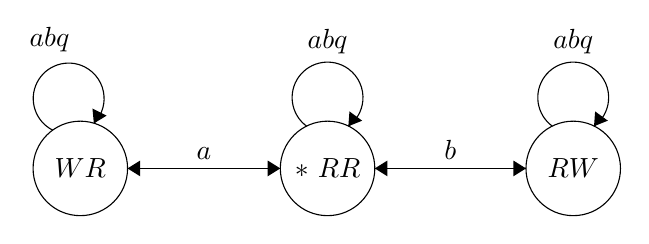
\begin{tikzpicture}[scale=0.2]
    \tikzstyle{every node}+=[inner sep=0pt]
    \draw [black] (38.4,-13.7) circle (3);
    \draw (38.4,-13.7) node {$*\mbox{ }RR$};
    \draw [black] (54,-13.7) circle (3);
    \draw (54,-13.7) node {$RW$};
    \draw [black] (22.7,-13.7) circle (3);
    \draw (22.7,-13.7) node {$WR$};
    \draw [black] (41.4,-13.7) -- (51,-13.7);
    \fill [black] (51,-13.7) -- (50.2,-13.2) -- (50.2,-14.2);
    \draw (46.2,-13.2) node [above] {$b$};
    \draw [black] (51,-13.7) -- (41.4,-13.7);
    \fill [black] (41.4,-13.7) -- (42.2,-14.2) -- (42.2,-13.2);
    \draw [black] (35.4,-13.7) -- (25.7,-13.7);
    \fill [black] (25.7,-13.7) -- (26.5,-14.2) -- (26.5,-13.2);
    \draw (30.55,-13.2) node [above] {$a$};
    \draw [black] (25.7,-13.7) -- (35.4,-13.7);
    \fill [black] (35.4,-13.7) -- (34.6,-13.2) -- (34.6,-14.2);
    \draw [black] (37.077,-11.02) arc (234:-54:2.25);
    \draw (38.4,-6.45) node [above] {$abq$};
    \fill [black] (39.72,-11.02) -- (40.6,-10.67) -- (39.79,-10.08);
    \draw [black] (52.677,-11.02) arc (234:-54:2.25);
    \draw (54,-6.45) node [above] {$abq$};
    \fill [black] (55.32,-11.02) -- (56.2,-10.67) -- (55.39,-10.08);
    \draw [black] (20.955,-11.274) arc (243.46232:-44.53768:2.25);
    \draw (20.74,-6.36) node [above] {$abq$};
    \fill [black] (23.56,-10.84) -- (24.37,-10.35) -- (23.47,-9.9);
    \end{tikzpicture}
    \end{center}

    This is an epistemic model: YES \\

    \pagebreak

    \item Seperately a and b look in their mirrors and see their red hats, the
    queen sees everything, represented in the event model $\Sigma$ with four
    actions: \\

    \begin{center}
    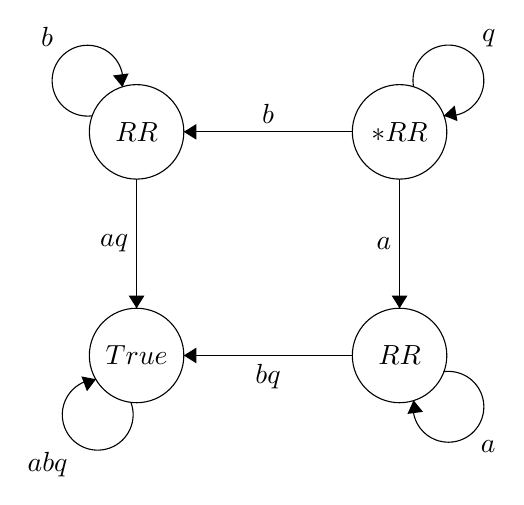
\begin{tikzpicture}[scale=0.2]
    \tikzstyle{every node}+=[inner sep=0pt]
    \draw [black] (54,-42.2) circle (3);
    \draw (54,-42.2) node {$RR$};
    \draw [black] (37.3,-28) circle (3);
    \draw (37.3,-28) node {$RR$};
    \draw [black] (37.3,-42.2) circle (3);
    \draw (37.3,-42.2) node {$True$};
    \draw [black] (54,-28) circle (3);
    \draw (54,-28) node {$*RR$};
    \draw [black] (56.805,-43.229) arc (97.58097:-190.41903:2.25);
    \draw (59.62,-47.57) node [below] {$a$};
    \fill [black] (54.89,-45.05) -- (54.5,-45.91) -- (55.49,-45.78);
    \draw [black] (34.491,-26.979) arc (277.76012:-10.23988:2.25);
    \draw (31.61,-22.64) node [above] {$b$};
    \fill [black] (36.4,-25.15) -- (36.79,-24.29) -- (35.8,-24.42);
    \draw [black] (51,-42.2) -- (40.3,-42.2);
    \fill [black] (40.3,-42.2) -- (41.1,-42.7) -- (41.1,-41.7);
    \draw (45.65,-42.7) node [below] {$bq$};
    \draw [black] (37.3,-31) -- (37.3,-39.2);
    \fill [black] (37.3,-39.2) -- (37.8,-38.4) -- (36.8,-38.4);
    \draw (36.8,-35.1) node [left] {$aq$};
    \draw [black] (51,-28) -- (40.3,-28);
    \fill [black] (40.3,-28) -- (41.1,-28.5) -- (41.1,-27.5);
    \draw (45.65,-27.5) node [above] {$b$};
    \draw [black] (54,-31) -- (54,-39.2);
    \fill [black] (54,-39.2) -- (54.5,-38.4) -- (53.5,-38.4);
    \draw (53.5,-35.1) node [left] {$a$};
    \draw [black] (54.889,-25.147) arc (190.43418:-97.56582:2.25);
    \draw (59.67,-22.63) node [above] {$q$};
    \fill [black] (56.81,-26.97) -- (57.68,-27.32) -- (57.5,-26.33);
    \draw [black] (36.935,-45.166) arc (20.7166:-267.2834:2.25);
    \draw (31.65,-48.34) node [below] {$abq$};
    \fill [black] (34.72,-43.71) -- (33.8,-43.53) -- (34.15,-44.47);
    \end{tikzpicture}
    \end{center}

    This is an epistemic model: NO \\
    This is a doxasic model: YES \\

    \item The update product of the two models \textbf{M}
    $\bigotimes$ $\Sigma$ : \\

    \begin{center}
    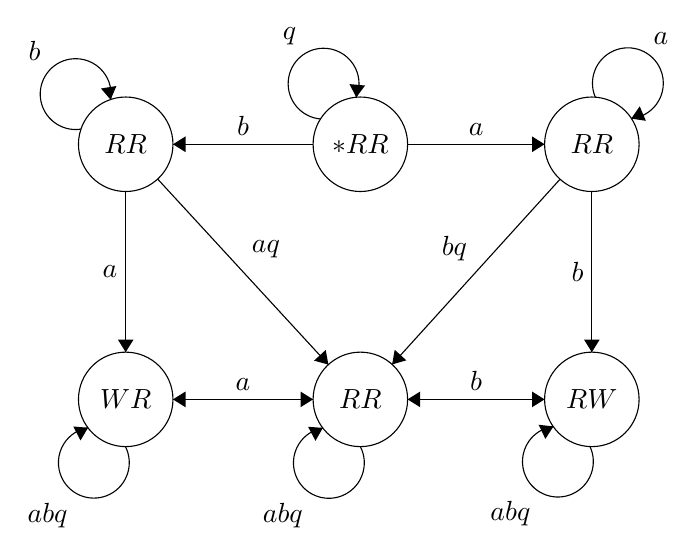
\begin{tikzpicture}[scale=0.2]
    \tikzstyle{every node}+=[inner sep=0pt]
    \draw [black] (8.5,-48.9) circle (3);
    \draw (8.5,-48.9) node {$WR$};
    \draw [black] (23.4,-48.9) circle (3);
    \draw (23.4,-48.9) node {$RR$};
    \draw [black] (38.1,-48.9) circle (3);
    \draw (38.1,-48.9) node {$RW$};
    \draw [black] (8.5,-32.7) circle (3);
    \draw (8.5,-32.7) node {$RR$};
    \draw [black] (23.4,-32.7) circle (3);
    \draw (23.4,-32.7) node {$*RR$};
    \draw [black] (38.1,-32.7) circle (3);
    \draw (38.1,-32.7) node {$RR$};
    \draw [black] (8.476,-51.888) arc (27.27123:-260.72877:2.25);
    \draw (3.54,-55.44) node [below] {$abq$};
    \fill [black] (6.11,-50.7) -- (5.17,-50.62) -- (5.63,-51.51);
    \draw [black] (23.394,-51.888) arc (27.62144:-260.37856:2.25);
    \draw (18.48,-55.46) node [below] {$abq$};
    \fill [black] (21.02,-50.71) -- (20.08,-50.64) -- (20.55,-51.53);
    \draw [black] (37.977,-51.886) arc (25.36938:-262.63062:2.25);
    \draw (32.93,-55.33) node [below] {$abq$};
    \fill [black] (35.66,-50.62) -- (34.72,-50.51) -- (35.15,-51.41);
    \draw [black] (26.4,-48.9) -- (35.1,-48.9);
    \fill [black] (35.1,-48.9) -- (34.3,-48.4) -- (34.3,-49.4);
    \draw (30.75,-48.4) node [above] {$b$};
    \draw [black] (20.4,-48.9) -- (11.5,-48.9);
    \fill [black] (11.5,-48.9) -- (12.3,-49.4) -- (12.3,-48.4);
    \draw (15.95,-48.4) node [above] {$a$};
    \draw [black] (11.5,-48.9) -- (20.4,-48.9);
    \fill [black] (20.4,-48.9) -- (19.6,-48.4) -- (19.6,-49.4);
    \draw [black] (35.1,-48.9) -- (26.4,-48.9);
    \fill [black] (26.4,-48.9) -- (27.2,-49.4) -- (27.2,-48.4);
    \draw [black] (8.5,-35.7) -- (8.5,-45.9);
    \fill [black] (8.5,-45.9) -- (9,-45.1) -- (8,-45.1);
    \draw (8,-40.8) node [left] {$a$};
    \draw [black] (5.671,-31.737) arc (278.9367:-9.0633:2.25);
    \draw (2.71,-27.44) node [above] {$b$};
    \fill [black] (7.54,-29.87) -- (7.91,-29) -- (6.93,-29.16);
    \draw [black] (20.4,-32.7) -- (11.5,-32.7);
    \fill [black] (11.5,-32.7) -- (12.3,-33.2) -- (12.3,-32.2);
    \draw (15.95,-32.2) node [above] {$b$};
    \draw [black] (20.879,-31.095) arc (265.25323:-22.74677:2.25);
    \draw (18.9,-26.43) node [above] {$q$};
    \fill [black] (23.14,-29.72) -- (23.7,-28.97) -- (22.71,-28.88);
    \draw [black] (26.4,-32.7) -- (35.1,-32.7);
    \fill [black] (35.1,-32.7) -- (34.3,-32.2) -- (34.3,-33.2);
    \draw (30.75,-32.2) node [above] {$a$};
    \draw [black] (38.325,-29.72) arc (203.42077:-84.57923:2.25);
    \draw (42.48,-26.39) node [above] {$a$};
    \fill [black] (40.6,-31.07) -- (41.53,-31.21) -- (41.14,-30.29);
    \draw [black] (38.1,-35.7) -- (38.1,-45.9);
    \fill [black] (38.1,-45.9) -- (38.6,-45.1) -- (37.6,-45.1);
    \draw (37.6,-40.8) node [left] {$b$};
    \draw [black] (10.53,-34.91) -- (21.37,-46.69);
    \fill [black] (21.37,-46.69) -- (21.2,-45.76) -- (20.46,-46.44);
    \draw (16.48,-39.34) node [right] {$aq$};
    \draw [black] (36.08,-34.92) -- (25.42,-46.68);
    \fill [black] (25.42,-46.68) -- (26.32,-46.42) -- (25.58,-45.75);
    \draw (30.21,-39.34) node [left] {$bq$};
    \end{tikzpicture}
    \end{center}

    This is an epistemic model: NO \\
    This is a doxasic model: YES \\

\end{enumerate}


%%%%%%%%%%%%%%%%
%% Exercise 2 %%
%%%%%%%%%%%%%%%%
\section*{Exercise 2}

\begin{enumerate}

    \item Representation of the bits world as an epistemic model \textbf{M}: \\

    \begin{center}
    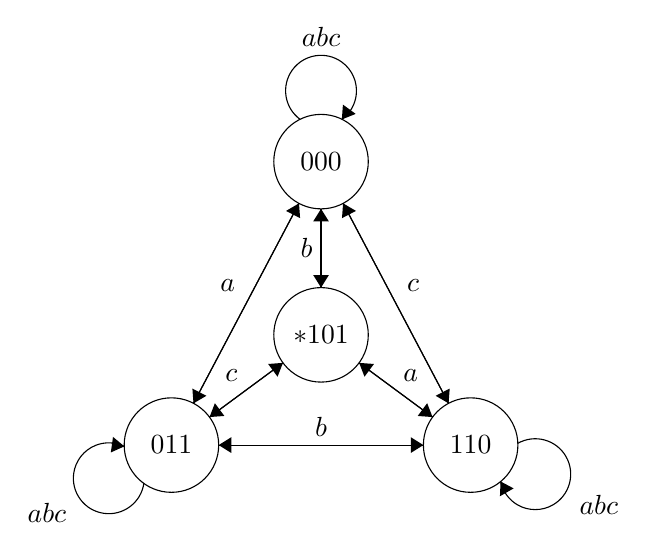
\begin{tikzpicture}[scale=0.2]
    \tikzstyle{every node}+=[inner sep=0pt]
    \draw [black] (39.9,-16.8) circle (3);
    \draw (39.9,-16.8) node {$000$};
    \draw [black] (39.9,-27.8) circle (3);
    \draw (39.9,-27.8) node {$*101$};
    \draw [black] (49.4,-34.8) circle (3);
    \draw (49.4,-34.8) node {$110$};
    \draw [black] (30.4,-34.8) circle (3);
    \draw (30.4,-34.8) node {$011$};
    \draw [black] (28.65,-37.223) arc (-8.10273:-296.10273:2.25);
    \draw (23.75,-39.12) node [left] {$abc$};
    \fill [black] (27.41,-34.88) -- (26.69,-34.28) -- (26.55,-35.27);
    \draw [black] (52.386,-34.694) arc (119.76798:-168.23202:2.25);
    \draw (56.28,-38.57) node [right] {$abc$};
    \fill [black] (51.3,-37.11) -- (51.26,-38.05) -- (52.13,-37.55);
    \draw [black] (38.577,-14.12) arc (234:-54:2.25);
    \draw (39.9,-9.55) node [above] {$abc$};
    \fill [black] (41.22,-14.12) -- (42.1,-13.77) -- (41.29,-13.18);
    \draw [black] (31.8,-32.15) -- (38.5,-19.45);
    \fill [black] (38.5,-19.45) -- (37.68,-19.93) -- (38.57,-20.39);
    \draw (34.47,-24.64) node [left] {$a$};
    \draw [black] (38.5,-19.45) -- (31.8,-32.15);
    \fill [black] (31.8,-32.15) -- (32.62,-31.67) -- (31.73,-31.21);
    \draw [black] (33.4,-34.8) -- (46.4,-34.8);
    \fill [black] (46.4,-34.8) -- (45.6,-34.3) -- (45.6,-35.3);
    \draw [black] (46.4,-34.8) -- (33.4,-34.8);
    \fill [black] (33.4,-34.8) -- (34.2,-35.3) -- (34.2,-34.3);
    \draw (39.9,-34.3) node [above] {$b$};
    \draw [black] (41.3,-19.45) -- (48,-32.15);
    \fill [black] (48,-32.15) -- (48.07,-31.21) -- (47.18,-31.67);
    \draw (45.33,-24.64) node [right] {$c$};
    \draw [black] (48,-32.15) -- (41.3,-19.45);
    \fill [black] (41.3,-19.45) -- (41.23,-20.39) -- (42.12,-19.93);
    \draw [black] (46.98,-33.02) -- (42.32,-29.58);
    \fill [black] (42.32,-29.58) -- (42.66,-30.46) -- (43.26,-29.65);
    \draw (45.6,-30.8) node [above] {$a$};
    \draw [black] (42.32,-29.58) -- (46.98,-33.02);
    \fill [black] (46.98,-33.02) -- (46.64,-32.14) -- (46.04,-32.95);
    \draw [black] (39.9,-24.8) -- (39.9,-19.8);
    \fill [black] (39.9,-19.8) -- (39.4,-20.6) -- (40.4,-20.6);
    \draw [black] (39.9,-19.8) -- (39.9,-24.8);
    \fill [black] (39.9,-24.8) -- (40.4,-24) -- (39.4,-24);
    \draw (39.4,-22.3) node [left] {$b$};
    \draw [black] (32.82,-33.02) -- (37.48,-29.58);
    \fill [black] (37.48,-29.58) -- (36.54,-29.65) -- (37.14,-30.46);
    \draw [black] (37.48,-29.58) -- (32.82,-33.02);
    \fill [black] (32.82,-33.02) -- (33.76,-32.95) -- (33.16,-32.14);
    \draw (34.2,-30.8) node [above] {$c$};
    \end{tikzpicture}
    \end{center}

    \item Representation of event model $\Sigma$:

    \begin{center}
    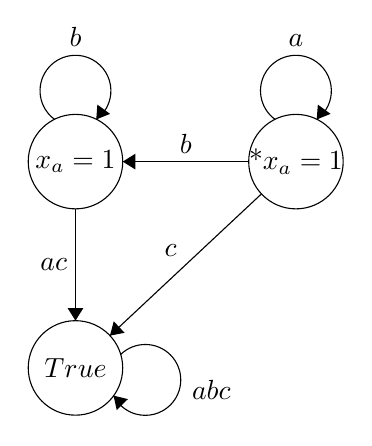
\begin{tikzpicture}[scale=0.2]
    \tikzstyle{every node}+=[inner sep=0pt]
    \draw [black] (17.2,-19.9) circle (3);
    \draw (17.2,-19.9) node {$x_a=1$};
    \draw [black] (17.2,-33) circle (3);
    \draw (17.2,-33) node {$True$};
    \draw [black] (31.2,-19.9) circle (3);
    \draw (31.2,-19.9) node {*$x_a=1$};
    \draw [black] (15.877,-17.22) arc (234:-54:2.25);
    \draw (17.2,-12.65) node [above] {$b$};
    \fill [black] (18.52,-17.22) -- (19.4,-16.87) -- (18.59,-16.28);
    \draw [black] (17.2,-22.9) -- (17.2,-30);
    \fill [black] (17.2,-30) -- (17.7,-29.2) -- (16.7,-29.2);
    \draw (16.7,-26.45) node [left] {$ac$};
    \draw [black] (29.877,-17.22) arc (234:-54:2.25);
    \draw (31.2,-12.65) node [above] {$a$};
    \fill [black] (32.52,-17.22) -- (33.4,-16.87) -- (32.59,-16.28);
    \draw [black] (28.2,-19.9) -- (20.2,-19.9);
    \fill [black] (20.2,-19.9) -- (21,-20.4) -- (21,-19.4);
    \draw (24.2,-19.4) node [above] {$b$};
    \draw [black] (29.01,-21.95) -- (19.39,-30.95);
    \fill [black] (19.39,-30.95) -- (20.32,-30.77) -- (19.63,-30.04);
    \draw (23.24,-25.97) node [above] {$c$};
    \draw [black] (20.065,-32.15) arc (134.26569:-153.73431:2.25);
    \draw (24.57,-34.38) node [right] {$abc$};
    \fill [black] (19.62,-34.76) -- (19.82,-35.68) -- (20.53,-34.98);
    \end{tikzpicture}
    \end{center}

    \pagebreak
    \item Representation of model \textbf{M'}:

    \begin{center}
    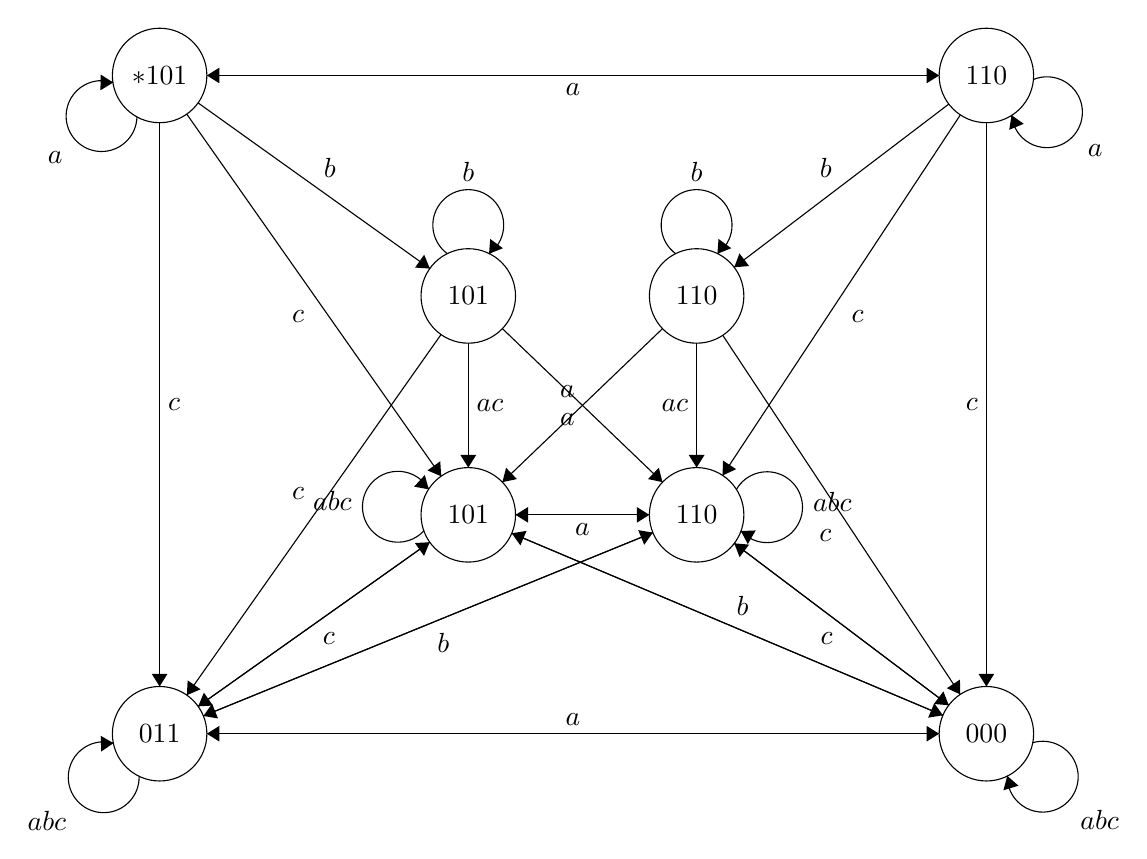
\begin{tikzpicture}[scale=0.2]
    \tikzstyle{every node}+=[inner sep=0pt]
    \draw [black] (65.3,-48.5) circle (3);
    \draw (65.3,-48.5) node {$000$};
    \draw [black] (32.4,-34.6) circle (3);
    \draw (32.4,-34.6) node {$101$};
    \draw [black] (46.9,-34.6) circle (3);
    \draw (46.9,-34.6) node {$110$};
    \draw [black] (12.8,-48.5) circle (3);
    \draw (12.8,-48.5) node {$011$};
    \draw [black] (32.4,-20.7) circle (3);
    \draw (32.4,-20.7) node {$101$};
    \draw [black] (46.9,-20.7) circle (3);
    \draw (46.9,-20.7) node {$110$};
    \draw [black] (65.3,-6.7) circle (3);
    \draw (65.3,-6.7) node {$110$};
    \draw [black] (12.8,-6.7) circle (3);
    \draw (12.8,-6.7) node {$*101$};
    \draw [black] (62.54,-47.33) -- (35.16,-35.77);
    \fill [black] (35.16,-35.77) -- (35.71,-36.54) -- (36.1,-35.62);
    \draw (49.82,-41.04) node [above] {$b$};
    \draw [black] (35.16,-35.77) -- (62.54,-47.33);
    \fill [black] (62.54,-47.33) -- (61.99,-46.56) -- (61.6,-47.48);
    \draw [black] (15.25,-46.76) -- (29.95,-36.34);
    \fill [black] (29.95,-36.34) -- (29.01,-36.39) -- (29.59,-37.21);
    \draw (23.55,-42.05) node [below] {$c$};
    \draw [black] (29.95,-36.34) -- (15.25,-46.76);
    \fill [black] (15.25,-46.76) -- (16.19,-46.71) -- (15.61,-45.89);
    \draw [black] (35.4,-34.6) -- (43.9,-34.6);
    \fill [black] (43.9,-34.6) -- (43.1,-34.1) -- (43.1,-35.1);
    \draw (39.65,-35.1) node [below] {$a$};
    \draw [black] (43.9,-34.6) -- (35.4,-34.6);
    \fill [black] (35.4,-34.6) -- (36.2,-35.1) -- (36.2,-34.1);
    \draw [black] (15.8,-48.5) -- (62.3,-48.5);
    \fill [black] (62.3,-48.5) -- (61.5,-48) -- (61.5,-49);
    \draw (39.05,-48) node [above] {$a$};
    \draw [black] (62.3,-48.5) -- (15.8,-48.5);
    \fill [black] (15.8,-48.5) -- (16.6,-49) -- (16.6,-48);
    \draw [black] (15.58,-47.37) -- (44.12,-35.73);
    \fill [black] (44.12,-35.73) -- (43.19,-35.57) -- (43.57,-36.5);
    \draw (30.81,-42.07) node [below] {$b$};
    \draw [black] (44.12,-35.73) -- (15.58,-47.37);
    \fill [black] (15.58,-47.37) -- (16.51,-47.53) -- (16.13,-46.6);
    \draw [black] (62.91,-46.69) -- (49.29,-36.41);
    \fill [black] (49.29,-36.41) -- (49.63,-37.29) -- (50.23,-36.49);
    \draw (55.15,-42.05) node [below] {$c$};
    \draw [black] (49.29,-36.41) -- (62.91,-46.69);
    \fill [black] (62.91,-46.69) -- (62.57,-45.81) -- (61.97,-46.61);
    \draw [black] (68.233,-49.073) arc (106.67475:-181.32525:2.25);
    \draw (71.24,-54) node [right] {$abc$};
    \fill [black] (66.63,-51.18) -- (66.38,-52.09) -- (67.34,-51.8);
    \draw [black] (11.497,-51.189) arc (1.88392:-286.11608:2.25);
    \draw (6.9,-54.06) node [left] {$abc$};
    \fill [black] (9.87,-49.1) -- (9.06,-48.63) -- (9.09,-49.63);
    \draw [black] (49.421,-32.996) arc (150.19:-137.81:2.25);
    \draw (54.26,-33.77) node [right] {$abc$};
    \fill [black] (49.71,-35.63) -- (50.15,-36.46) -- (50.65,-35.59);
    \draw [black] (29.587,-35.607) arc (317.43022:29.43022:2.25);
    \draw (25.03,-33.71) node [left] {$abc$};
    \fill [black] (29.89,-32.98) -- (29.64,-32.07) -- (28.96,-32.81);
    \draw [black] (34.57,-22.78) -- (44.73,-32.52);
    \fill [black] (44.73,-32.52) -- (44.5,-31.61) -- (43.81,-32.33);
    \draw (38.69,-28.13) node [below] {$a$};
    \draw [black] (45.577,-18.02) arc (234:-54:2.25);
    \draw (46.9,-13.45) node [above] {$b$};
    \fill [black] (48.22,-18.02) -- (49.1,-17.67) -- (48.29,-17.08);
    \draw [black] (44.73,-22.78) -- (34.57,-32.52);
    \fill [black] (34.57,-32.52) -- (35.49,-32.33) -- (34.8,-31.61);
    \draw (38.69,-27.17) node [above] {$a$};
    \draw [black] (31.077,-18.02) arc (234:-54:2.25);
    \draw (32.4,-13.45) node [above] {$b$};
    \fill [black] (33.72,-18.02) -- (34.6,-17.67) -- (33.79,-17.08);
    \draw [black] (32.4,-23.7) -- (32.4,-31.6);
    \fill [black] (32.4,-31.6) -- (32.9,-30.8) -- (31.9,-30.8);
    \draw (32.9,-27.65) node [right] {$ac$};
    \draw [black] (15.24,-8.44) -- (29.96,-18.96);
    \fill [black] (29.96,-18.96) -- (29.6,-18.08) -- (29.02,-18.9);
    \draw (23.6,-13.2) node [above] {$b$};
    \draw [black] (62.91,-8.52) -- (49.29,-18.88);
    \fill [black] (49.29,-18.88) -- (50.23,-18.8) -- (49.62,-18);
    \draw (55.1,-13.2) node [above] {$b$};
    \draw [black] (46.9,-23.7) -- (46.9,-31.6);
    \fill [black] (46.9,-31.6) -- (47.4,-30.8) -- (46.4,-30.8);
    \draw (46.4,-27.65) node [left] {$ac$};
    \draw [black] (68.277,-6.96) arc (112.73627:-175.26373:2.25);
    \draw (71.71,-11.47) node [right] {$a$};
    \fill [black] (66.9,-9.22) -- (66.75,-10.15) -- (67.67,-9.77);
    \draw [black] (11.361,-9.319) arc (-1.04687:-289.04687:2.25);
    \draw (6.67,-11.93) node [left] {$a$};
    \fill [black] (9.85,-7.15) -- (9.06,-6.64) -- (9.04,-7.64);
    \draw [black] (15.8,-6.7) -- (62.3,-6.7);
    \fill [black] (62.3,-6.7) -- (61.5,-6.2) -- (61.5,-7.2);
    \draw (39.05,-7.2) node [below] {$a$};
    \draw [black] (62.3,-6.7) -- (15.8,-6.7);
    \fill [black] (15.8,-6.7) -- (16.6,-7.2) -- (16.6,-6.2);
    \draw [black] (12.8,-9.7) -- (12.8,-45.5);
    \fill [black] (12.8,-45.5) -- (13.3,-44.7) -- (12.3,-44.7);
    \draw (13.3,-27.6) node [right] {$c$};
    \draw [black] (14.52,-9.15) -- (30.68,-32.15);
    \fill [black] (30.68,-32.15) -- (30.62,-31.2) -- (29.81,-31.78);
    \draw (22.01,-22.01) node [left] {$c$};
    \draw [black] (30.67,-23.15) -- (14.53,-46.05);
    \fill [black] (14.53,-46.05) -- (15.4,-45.68) -- (14.58,-45.11);
    \draw (22.01,-33.23) node [left] {$c$};
    \draw [black] (65.3,-9.7) -- (65.3,-45.5);
    \fill [black] (65.3,-45.5) -- (65.8,-44.7) -- (64.8,-44.7);
    \draw (64.8,-27.6) node [left] {$c$};
    \draw [black] (63.65,-9.2) -- (48.55,-32.1);
    \fill [black] (48.55,-32.1) -- (49.41,-31.7) -- (48.57,-31.15);
    \draw (56.71,-21.98) node [right] {$c$};
    \draw [black] (48.56,-23.2) -- (63.64,-46);
    \fill [black] (63.64,-46) -- (63.62,-45.06) -- (62.79,-45.61);
    \draw (55.49,-35.93) node [left] {$c$};
    \end{tikzpicture}
    \end{center}

    \item Representation of event model \textbf{$\Sigma$'}:
    
    \begin{center}
    	\begin{tikzpicture}[scale=0.2]
    	\tikzstyle{every node}+=[inner sep=0pt]
    	\draw [black] (38.9,-44.6) circle (3);
    	\draw (38.9,-44.6) node {$true$};
    	\draw [black] (24.9,-30.6) circle (3);
    	\draw (24.9,-30.6) node {$x_{a} = 1$};
    	\draw [black] (51.2,-30.6) circle (3);
    	\draw (51.2,-30.6) node {$x_{a} = 0$};
    	\draw [black] (24.9,-10.9) circle (3);
    	\draw (24.9,-10.9) node {$x_{a} = 1$};
    	\draw [black] (51.2,-10.9) circle (3);
    	\draw (51.2,-10.9) node {$x_{a} = 0$};
    	\draw [black] (23.577,-8.22) arc (234:-54:2.25);
    	\draw (24.9,-3.65) node [above] {$a,c$};
    	\fill [black] (26.22,-8.22) -- (27.1,-7.87) -- (26.29,-7.28);
    	\draw [black] (49.877,-8.22) arc (234:-54:2.25);
    	\draw (51.2,-3.65) node [above] {$a,c$};
    	\fill [black] (52.52,-8.22) -- (53.4,-7.87) -- (52.59,-7.28);
    	\draw [black] (27.9,-10.9) -- (48.2,-10.9);
    	\fill [black] (48.2,-10.9) -- (47.4,-10.4) -- (47.4,-11.4);
    	\draw [black] (48.2,-10.9) -- (27.9,-10.9);
    	\fill [black] (27.9,-10.9) -- (28.7,-11.4) -- (28.7,-10.4);
    	\draw (38.05,-10.4) node [above] {$c$};
    	\draw [black] (24.9,-13.9) -- (24.9,-27.6);
    	\fill [black] (24.9,-27.6) -- (25.4,-26.8) -- (24.4,-26.8);
    	\draw (24.4,-20.75) node [left] {$b$};
    	\draw [black] (51.2,-13.9) -- (51.2,-27.6);
    	\fill [black] (51.2,-27.6) -- (51.7,-26.8) -- (50.7,-26.8);
    	\draw (50.7,-20.75) node [left] {$b$};
    	\draw [black] (27.02,-32.72) -- (36.78,-42.48);
    	\fill [black] (36.78,-42.48) -- (36.57,-41.56) -- (35.86,-42.27);
    	\draw (30.24,-38.08) node [below] {$a,c$};
    	\draw [black] (49.22,-32.85) -- (40.88,-42.35);
    	\fill [black] (40.88,-42.35) -- (41.78,-42.08) -- (41.03,-41.42);
    	\draw (44.51,-36.15) node [left] {$a,c$};
    	\draw [black] (22.22,-31.923) arc (324:36:2.25);
    	\draw (17.65,-30.6) node [left] {$b$};
    	\fill [black] (22.22,-29.28) -- (21.87,-28.4) -- (21.28,-29.21);
    	\draw [black] (53.88,-29.277) arc (144:-144:2.25);
    	\draw (58.45,-30.6) node [right] {$b$};
    	\fill [black] (53.88,-31.92) -- (54.23,-32.8) -- (54.82,-31.99);
    	\end{tikzpicture}
    \end{center}

    \begin{center}
    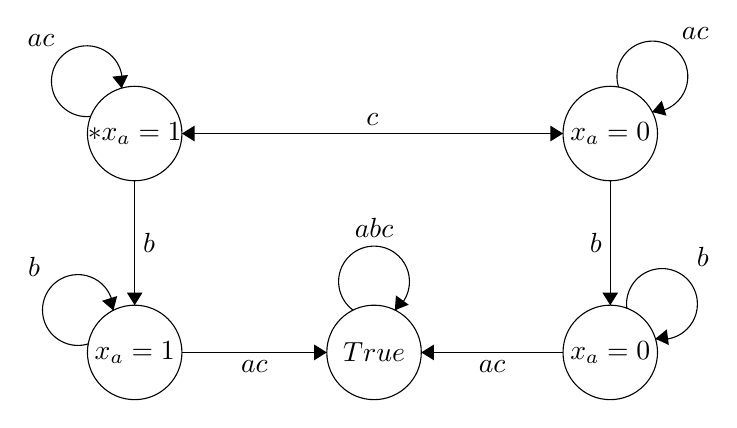
\begin{tikzpicture}[scale=0.2]
    \tikzstyle{every node}+=[inner sep=0pt]
    \draw [black] (18.3,-23.4) circle (3);
    \draw (18.3,-23.4) node {$x_a=1$};
    \draw [black] (48.5,-9.5) circle (3);
    \draw (48.5,-9.5) node {$x_a=0$};
    \draw [black] (33.5,-23.4) circle (3);
    \draw (33.5,-23.4) node {$True$};
    \draw [black] (18.3,-9.5) circle (3);
    \draw (18.3,-9.5) node {$*x_a=1$};
    \draw [black] (48.5,-23.4) circle (3);
    \draw (48.5,-23.4) node {$x_a=0$};
    \draw [black] (15.362,-22.855) arc (287.21852:-0.78148:2.25);
    \draw (12.32,-17.96) node [left] {$b$};
    \fill [black] (16.95,-20.74) -- (17.19,-19.82) -- (16.23,-20.12);
    \draw [black] (49.029,-6.559) arc (197.52793:-90.47207:2.25);
    \draw (53.9,-3.57) node [above] {$ac$};
    \fill [black] (51.16,-8.13) -- (52.07,-8.37) -- (51.77,-7.41);
    \draw [black] (32.177,-20.72) arc (234:-54:2.25);
    \draw (33.5,-16.15) node [above] {$abc$};
    \fill [black] (34.82,-20.72) -- (35.7,-20.37) -- (34.89,-19.78);
    \draw [black] (21.3,-23.4) -- (30.5,-23.4);
    \fill [black] (30.5,-23.4) -- (29.7,-22.9) -- (29.7,-23.9);
    \draw (25.9,-23.9) node [below] {$ac$};
    \draw [black] (18.3,-12.5) -- (18.3,-20.4);
    \fill [black] (18.3,-20.4) -- (18.8,-19.6) -- (17.8,-19.6);
    \draw (18.8,-16.45) node [right] {$b$};
    \draw [black] (15.516,-8.413) arc (276.39744:-11.60256:2.25);
    \draw (12.35,-4.03) node [above] {$ac$};
    \fill [black] (17.47,-6.63) -- (17.88,-5.78) -- (16.88,-5.89);
    \draw [black] (21.3,-9.5) -- (45.5,-9.5);
    \fill [black] (45.5,-9.5) -- (44.7,-9) -- (44.7,-10);
    \draw [black] (45.5,-9.5) -- (21.3,-9.5);
    \fill [black] (21.3,-9.5) -- (22.1,-10) -- (22.1,-9);
    \draw (33.4,-9) node [above] {$c$};
    \draw [black] (48.5,-12.5) -- (48.5,-20.4);
    \fill [black] (48.5,-20.4) -- (49,-19.6) -- (48,-19.6);
    \draw (48,-16.45) node [left] {$b$};
    \draw [black] (49.552,-20.603) arc (187.12:-100.88:2.25);
    \draw (53.96,-17.32) node [right] {$b$};
    \fill [black] (51.36,-22.53) -- (52.22,-22.93) -- (52.09,-21.94);
    \draw [black] (45.5,-23.4) -- (36.5,-23.4);
    \fill [black] (36.5,-23.4) -- (37.3,-23.9) -- (37.3,-22.9);
    \draw (41,-23.9) node [below] {$ac$};
    \end{tikzpicture}
    \end{center}

    \item The update product of the two models \textbf{M''} = \textbf{M}
    $\bigotimes$ \textbf{$\Sigma$'} : \\

\end{enumerate}


%%%%%%%%%%%%%%%%
%% Exercise 3 %%
%%%%%%%%%%%%%%%%
\section*{Exercise 3}

\begin{enumerate}

    \item \textit{How many possible worlds} are there (that are consistent with the story above)?\\
    \begin{center}
    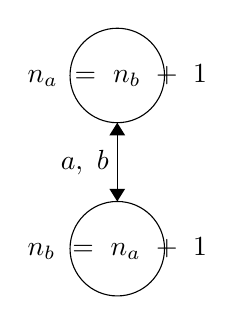
\begin{tikzpicture}[scale=0.2]
    \tikzstyle{every node}+=[inner sep=0pt]
    \draw [black] (44,-12.6) circle (3);
    \draw (44,-12.6) node {$n_{a}\mbox{ }=\mbox{ }n_{b}\mbox{ }+\mbox{ }1$};
    \draw [black] (44,-23.6) circle (3);
    \draw (44,-23.6) node {$n_{b}\mbox{ }=\mbox{ }n_{a}\mbox{ }+\mbox{ }1$};
    \draw [black] (44,-15.6) -- (44,-20.6);
    \fill [black] (44,-20.6) -- (44.5,-19.8) -- (43.5,-19.8);
    \draw (43.5,-18.1) node [left] {$a,\mbox{ }b$};
    \draw [black] (44,-20.6) -- (44,-15.6);
    \fill [black] (44,-15.6) -- (43.5,-16.4) -- (44.5,-16.4);
    \end{tikzpicture}
    \end{center}

    \item Represent (draw) the above situation as an epistemic model M1, with two agents (a for Alice, b for Bob),  using pairs of numbers (na,nb) as “names” for the possible worlds. Draw the epistemic accessibility  relations for each agent. but  do
    not worry about the valuation (yet), since no atomic sentences are given yet.\\

    \begin{center}
    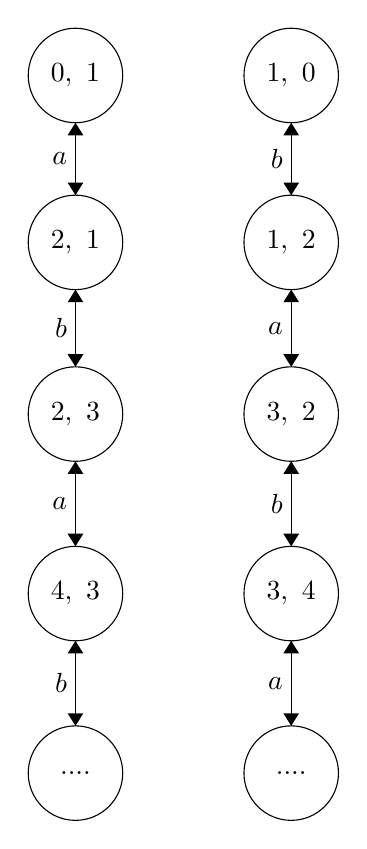
\begin{tikzpicture}[scale=0.2]
    \tikzstyle{every node}+=[inner sep=0pt]
    \draw [black] (25,-11.7) circle (3);
    \draw (25,-11.7) node {$0,\mbox{ }1$};
    \draw [black] (38.7,-11.7) circle (3);
    \draw (38.7,-11.7) node {$1,\mbox{ }0$};
    \draw [black] (38.7,-22.3) circle (3);
    \draw (38.7,-22.3) node {$1,\mbox{ }2$};
    \draw [black] (25,-22.3) circle (3);
    \draw (25,-22.3) node {$2,\mbox{ }1$};
    \draw [black] (25,-33.2) circle (3);
    \draw (25,-33.2) node {$2,\mbox{ }3$};
    \draw [black] (38.7,-33.2) circle (3);
    \draw (38.7,-33.2) node {$3,\mbox{ }2$};
    \draw [black] (25,-44.6) circle (3);
    \draw (25,-44.6) node {$4,\mbox{ }3$};
    \draw [black] (38.7,-44.6) circle (3);
    \draw (38.7,-44.6) node {$3,\mbox{ }4$};
    \draw [black] (25,-56) circle (3);
    \draw (25,-56) node {$....$};
    \draw [black] (38.7,-56) circle (3);
    \draw (38.7,-56) node {$....$};
    \draw [black] (25,-14.7) -- (25,-19.3);
    \fill [black] (25,-19.3) -- (25.5,-18.5) -- (24.5,-18.5);
    \draw (24.5,-17) node [left] {$a$};
    \draw [black] (38.7,-14.7) -- (38.7,-19.3);
    \fill [black] (38.7,-19.3) -- (39.2,-18.5) -- (38.2,-18.5);
    \draw (38.2,-17) node [left] {$b$};
    \draw [black] (38.7,-25.3) -- (38.7,-30.2);
    \fill [black] (38.7,-30.2) -- (39.2,-29.4) -- (38.2,-29.4);
    \draw (38.2,-27.75) node [left] {$a$};
    \draw [black] (25,-25.3) -- (25,-30.2);
    \fill [black] (25,-30.2) -- (25.5,-29.4) -- (24.5,-29.4);
    \draw (24.5,-27.75) node [left] {$b$};
    \draw [black] (38.7,-36.2) -- (38.7,-41.6);
    \fill [black] (38.7,-41.6) -- (39.2,-40.8) -- (38.2,-40.8);
    \draw (38.2,-38.9) node [left] {$b$};
    \draw [black] (38.7,-47.6) -- (38.7,-53);
    \fill [black] (38.7,-53) -- (39.2,-52.2) -- (38.2,-52.2);
    \draw (38.2,-50.3) node [left] {$a$};
    \draw [black] (25,-47.6) -- (25,-53);
    \fill [black] (25,-53) -- (25.5,-52.2) -- (24.5,-52.2);
    \draw (24.5,-50.3) node [left] {$b$};
    \draw [black] (25,-36.2) -- (25,-41.6);
    \fill [black] (25,-41.6) -- (25.5,-40.8) -- (24.5,-40.8);
    \draw (24.5,-38.9) node [left] {$a$};
    \draw [black] (25,-19.3) -- (25,-14.7);
    \fill [black] (25,-14.7) -- (24.5,-15.5) -- (25.5,-15.5);
    \draw [black] (38.7,-19.3) -- (38.7,-14.7);
    \fill [black] (38.7,-14.7) -- (38.2,-15.5) -- (39.2,-15.5);
    \draw [black] (38.7,-30.2) -- (38.7,-25.3);
    \fill [black] (38.7,-25.3) -- (38.2,-26.1) -- (39.2,-26.1);
    \draw [black] (25,-30.2) -- (25,-25.3);
    \fill [black] (25,-25.3) -- (24.5,-26.1) -- (25.5,-26.1);
    \draw [black] (25,-41.6) -- (25,-36.2);
    \fill [black] (25,-36.2) -- (24.5,-37) -- (25.5,-37);
    \draw [black] (38.7,-41.6) -- (38.7,-36.2);
    \fill [black] (38.7,-36.2) -- (38.2,-37) -- (39.2,-37);
    \draw [black] (38.7,-53) -- (38.7,-47.6);
    \fill [black] (38.7,-47.6) -- (38.2,-48.4) -- (39.2,-48.4);
    \draw [black] (25,-53) -- (25,-47.6);
    \fill [black] (25,-47.6) -- (24.5,-48.4) -- (25.5,-48.4);
    \end{tikzpicture}
    \end{center}

    \item
    \item
    \item
    \item
    \item
    \item
    \item

\end{enumerate}


\end{document}


